% Borg: extended abstract for Vulkanised 2027 (2 pages).
\documentclass[sigconf,nonacm]{acmart}

\usepackage{booktabs}
\usepackage{microtype}
\usepackage{tikz}
\usetikzlibrary{positioning,fit,arrows.meta}

\settopmatter{printfolios=true}

\begin{document}

\title{Borg: Vulkan from vkcube Down to the Gates}

\author{Andreas Wendleder}
\orcid{0009-0008-8304-2818}
\affiliation{%
  \institution{Independent Researcher}
  \city{Landshut}
  \country{Germany}
}
\email{andreas.wendleder@proton.me}

\begin{abstract}
Borg is an open-source GPU: Chisel RTL for a small FP32 shader core that
runs 2x2 quads, with a tile-based rasterizer, a descriptor-based texture
unit and MSAA, aimed at an ECP5 FPGA and a GF180 ASIC. Its Vulkan driver,
borgvk, is a native Mesa ICD with its own NIR-based shader compiler.
Unmodified Khronos vkcube renders on the FPGA, also self-hosted on Linux
running on the board itself. This paper follows Vulkan~1.0 down to the
gates: which API features forced hardware into the design, how a driver
and compiler fit a GPU with 32 registers per lane, and how we run the
Vulkan CTS directly against the RTL with a compiled simulator to find
hardware bugs before tapeout.
\end{abstract}

\maketitle

\begin{figure}[t]
  \centering
  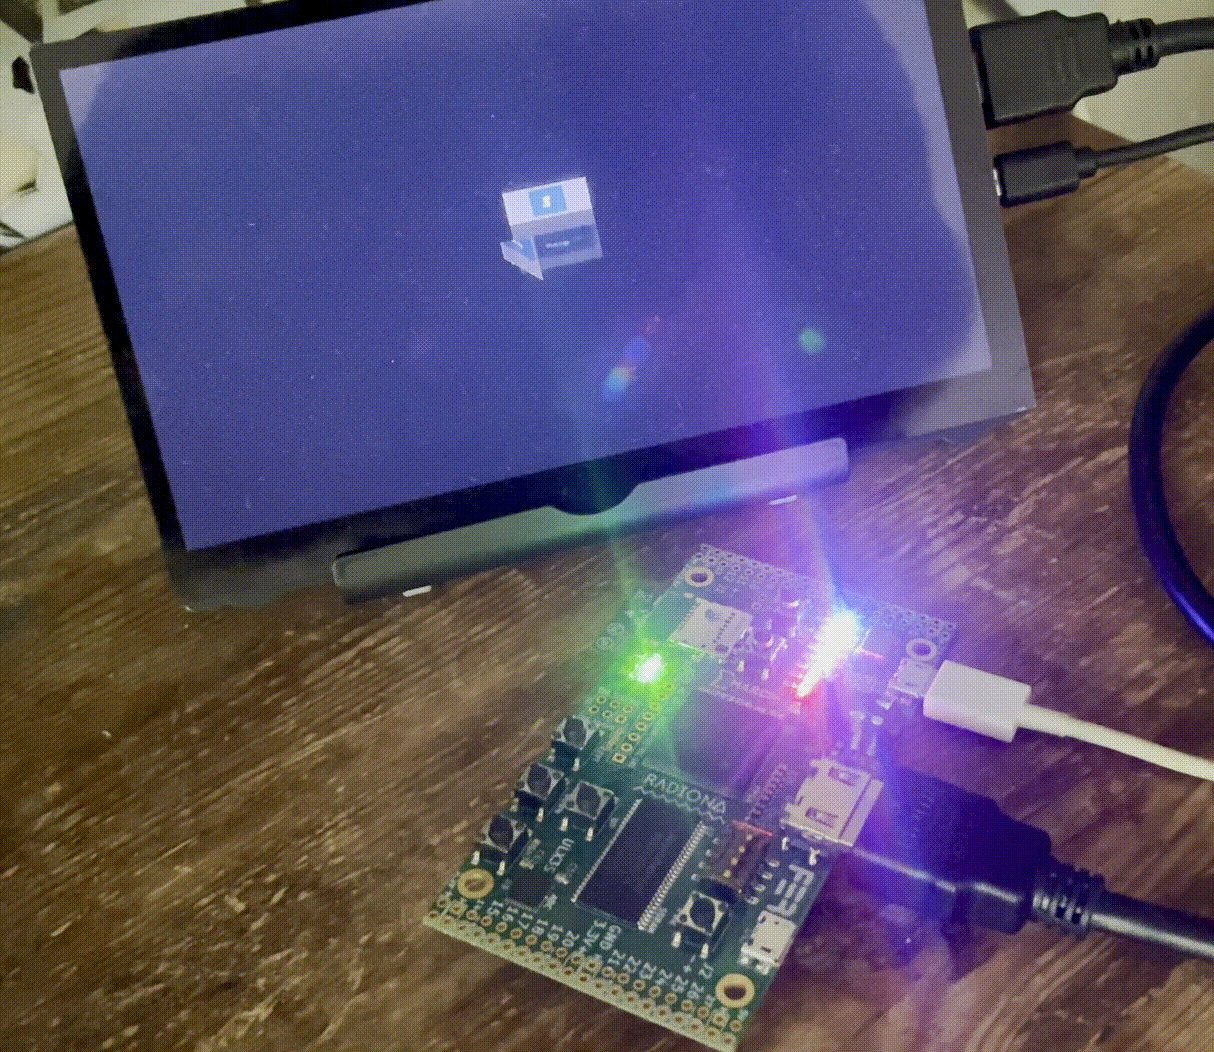
\includegraphics[width=0.8\columnwidth]{vkcube_ulx3s.jpg}
  \caption{The unmodified Khronos \texttt{cube.c} rendered by Borg on a
    ULX3S board (Lattice ECP5-85K), shown over HDMI.}
  \Description{Photo of a ULX3S FPGA board connected by HDMI to a small
    display showing the textured Vulkan cube.}
  \label{fig:teaser}
\end{figure}

\section{Introduction}

Borg is a GPU small enough for one person to read end to end: about
14,000 lines of Chisel for the GPU, a RISC-V CPU (Hutt) for the system
around it, and a Vulkan driver in Mesa. The same Chisel source targets the
ULX3S FPGA board and a GF180MCU ASIC slot on wafer.space. Everything is
open source.\footnote{\url{https://github.com/gonsolo/Borg}, documentation
at \url{https://gonsolo.github.io/Borg/}.}

The goal is not speed but completeness: a GPU that implements what
Vulkan~1.0 actually requires, and a driver that runs real applications,
starting with the unmodified Khronos \texttt{cube.c}
(Figure~\ref{fig:teaser}). Figure~\ref{fig:stack} shows the stack. The
driver, borgvk, is a native Mesa ICD modelled on v3dv: it uses Mesa's
Vulkan runtime and compiles SPIR-V through NIR to Borg's ISA. Its output is
a stream of command packets, which reaches one of three back ends: the FPGA
over a serial link; a DRM driver under Linux on the board's own CPU, where
\texttt{cube.c} runs with no host computer at all; or a compiled simulator
of the RTL that runs the Vulkan conformance test suite (CTS). The driver
code is the same in all three cases.

\begin{figure}[t]
  \centering
  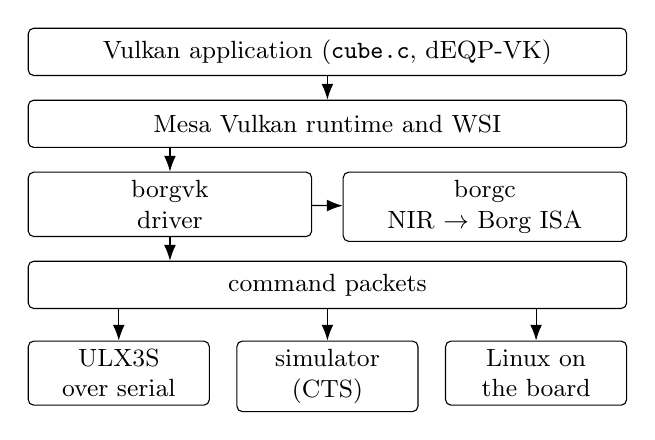
\begin{tikzpicture}[
      box/.style={draw, rounded corners=2pt, align=center, font=\small,
                  minimum height=6mm, inner sep=3pt},
      arr/.style={-{Latex[length=2mm]}}]
    \node[box, minimum width=7.6cm] (app) {Vulkan application (\texttt{cube.c}, dEQP-VK)};
    \node[box, minimum width=7.6cm, below=3mm of app] (rt) {Mesa Vulkan runtime and WSI};
    \node[box, minimum width=3.6cm, below=3mm of rt.south west, anchor=north west] (vk)
      {borgvk\\driver};
    \node[box, minimum width=3.6cm, below=3mm of rt.south east, anchor=north east] (cc)
      {borgc\\NIR $\rightarrow$ Borg ISA};
    \node[box, minimum width=7.6cm, below=3mm of vk.south west, anchor=north west] (pk)
      {command packets};
    \node[box, below=4mm of pk.south west, anchor=north west, minimum width=2.3cm] (fp)
      {ULX3S\\over serial};
    \node[box, below=4mm of pk.south, minimum width=2.3cm] (ds)
      {simulator\\(CTS)};
    \node[box, below=4mm of pk.south east, anchor=north east, minimum width=2.3cm] (sh)
      {Linux on\\the board};
    \draw[arr] (app) -- (rt);
    \draw[arr] (rt.south -| vk) -- (vk);
    \draw[arr] (vk) -- (cc);
    \draw[arr] (vk.south) -- (vk.south |- pk.north);
    \draw[arr] (pk.south -| fp) -- (fp);
    \draw[arr] (pk) -- (ds);
    \draw[arr] (pk.south -| sh) -- (sh);
  \end{tikzpicture}
  \caption{One driver, three back ends. All three consume the same packet
    stream; the simulator runs the RTL itself.}
  \Description{Block diagram: a Vulkan application on Mesa's runtime, the
    borgvk driver and the borgc compiler, a packet stream, and three back
    ends: the FPGA over serial, the simulator, and Linux on the board.}
  \label{fig:stack}
\end{figure}

\section{What Vulkan~1.0 asks of hardware}

Several features of Borg exist only because the API demanded them
(Table~\ref{tab:features}). Each was cheaper to build than to work around.

\begin{table}[t]
  \caption{Vulkan~1.0 requirements and the Borg hardware behind them.}
  \label{tab:features}
  \small
  \begin{tabular}{p{0.38\columnwidth}p{0.54\columnwidth}}
    \toprule
    Requirement & Borg mechanism \\
    \midrule
    Compute on every graphics queue & workgroup dispatch, \texttt{BARRIER}, atomics \\
    Derivatives, implicit LOD & 2x2 quad on four lanes \\
    Sampled images, samplers & descriptor-table texture unit: 51 formats, mipmaps, all address modes \\
    Colour attachment formats & raw attachments, blend by read-back \\
    Depth, stencil, scissor, blend & fixed function in the tile pipeline \\
    Occlusion queries & exact passing-sample counts \\
    4x MSAA & multi-pass per tile, about 9\% less area \\
    Vertex input, topologies & hardware draw front end \\
    \bottomrule
  \end{tabular}
\end{table}

\paragraph{A graphics queue implies compute.}
Vulkan~1.0 requires every queue family with graphics to support compute.
Borg therefore dispatches workgroups on the same shader core, with a
\texttt{BARRIER} instruction and atomics. This turned out to matter far
beyond compute applications: every \texttt{glsl.builtin.precision} case in
the CTS runs its shaders as compute dispatches, so the compute path gates
thousands of shader tests.

\paragraph{Derivatives need quads.}
\texttt{dFdx} and \texttt{dFdy} are differences between neighbouring
pixels, so the fragment core runs a 2x2 quad on four lanes, and implicit
LOD in the texture unit uses the same quad. A one-lane core would be
smaller and would return zero derivatives.

\paragraph{The draw front end.}
A single register write renders a whole draw: primitive assembly for
lists, strips, fans, indices, restart and instancing; one vertex shader run
per triangle; varyings written and read back by two instructions; and a
homogeneous 2D setup that needs no clipping, because vertices behind the
eye are handled exactly.

\section{A driver and compiler for 32 registers}

borgvk builds on Mesa's Vulkan runtime for objects, synchronization and
WSI; what is specific to Borg is the target. Its compiler, borgc, consumes
NIR after Mesa's standard lowering.
One instruction selector serves graphics and compute. The core has 32
registers per lane; constants live in a small uniform window that an
instruction can read as one of its operands, so the compiler places
constants in a pool and preloads what does not fit. Branches are
PC-relative, so code does not depend on where it is loaded. Where a shader
cannot be compiled correctly yet, borgc refuses it instead of guessing; a
refused pipeline is an honest CTS failure, while a miscompiled one can
pass by luck and fail later.

Two design decisions keep this manageable. The ISA lives in one file in
the format of the RISC-V \texttt{riscv-opcodes} project
(Listing~\ref{lst:opcodes}), from which the hardware decoder, the C
header and the compiler's encoder are generated. And every compiler change
is checked against a corpus: recorded shaders are recompiled, and a change
that should be a pure refactoring must produce identical binaries.

\begin{figure}[t]
\small
\begin{verbatim}
fmadd  rd rs1 rs2 rs3 f3  26..25=0 6..0=0x04
tex    rd rs1 rs2 rs3 f3  26..25=2 6..0=0x04
brnz   rs1 offset f3      31..25=0x28 6..0=0x00
\end{verbatim}
\caption{An excerpt of the opcode file. The decoder, the C header and the
  compiler's encoder are generated from it, so they cannot disagree.}
\Description{Three lines of an opcode table, each naming an instruction,
  its operand fields and its fixed bit ranges.}
\label{lst:opcodes}
\end{figure}

\section{Running the CTS against RTL}

An FPGA or a gate-level simulation is far too slow to run a conformance
suite with hundreds of thousands of cases. Borg's answer is a direct
simulator: the GPU's RTL, without CPU or firmware, compiled to native code
with CIRCT's arcilator, and driven by the same packet stream borgvk sends
to the board. It runs at roughly 140,000 to 230,000 cycles per second, and
many instances run in parallel. The CTS sees an ordinary Vulkan device.

Speed still decides what can be tested. The CTS shader-executor cases use
one invocation per workgroup, which left three of the four quad lanes idle;
packing four such workgroups into one quad cut an \texttt{atan2} vec4 case
from over 40 minutes to about two.

Running the CTS against the RTL finds bugs in all layers. Examples: the
texture unit returned one subtap instead of the average at cube corners in
\texttt{textureGather}, which surfaced against the CTS reference;
integer copies through a floating-point move were flushed to zero when
their bits looked like denormals; and branch targets in fragment programs
landed one word early. Each was found and fixed before silicon.

\begin{table}[t]
  \caption{Selected CTS results on the direct simulator (CTS 1.4.6.2).}
  \label{tab:cts}
  \small
  \begin{tabular}{lrrr}
    \toprule
    Scope & Cases & Pass & Fail \\
    \midrule
    \texttt{dEQP-VK.api} (2026-10-05) & 278,342 & 64,866 & 0 \\
    Graphics compiler corpus & 2,293 & 728 & 12 \\
    Compute compiler corpus & 3,990 & 3,711 & 258 \\
    \bottomrule
  \end{tabular}
\end{table}

Table~\ref{tab:cts} gives the current state. The \texttt{api} group runs
without failures, the remaining cases being optional features reported as
not supported. The compiler corpora (2026-10-20) are the CTS cases whose
shaders reach borgc; the cases neither passing nor failing are not supported
(graphics) or exceeded the 120\,s limit per case (compute). The full Vulkan~1.0 must-pass list does not pass yet; it is being
worked through group by group, with per-group results on the project's
status page.

\section{Lessons for a new implementation}

\begin{itemize}
  \item Bring up the \texttt{api} group first, and compute early: it is
    mandatory, and the precision tests depend on it.
  \item Make the simulator fast before chasing failures; test throughput
    sets the pace of everything else.
  \item Refuse what the compiler cannot do; silent miscompilation hides
    bugs the CTS would otherwise report.
  \item Keep one source of truth for the ISA; disagreements between copies
    caused several of the bugs above.
\end{itemize}

Next are the full Vulkan~1.0 must-pass list and a tapeout on wafer.space.

\begin{thebibliography}{6}
\bibitem{chisel} J.~Bachrach et al. Chisel: Constructing Hardware in a
  Scala Embedded Language. DAC 2012.
\bibitem{circt} CIRCT: Circuit IR Compilers and Tools.
  \url{https://circt.llvm.org}
\bibitem{cts} Khronos Group. Vulkan Conformance Test Suite (VK-GL-CTS).
  \url{https://github.com/KhronosGroup/VK-GL-CTS}
\bibitem{mesa} The Mesa 3D Graphics Library. \url{https://mesa3d.org}
\bibitem{riscvop} RISC-V International. riscv-opcodes.
  \url{https://github.com/riscv/riscv-opcodes}
\bibitem{ulx3s} Radiona. ULX3S FPGA board. \url{https://radiona.org/ulx3s/}
\end{thebibliography}

\end{document}
